\begin{figure}[h]
\centering
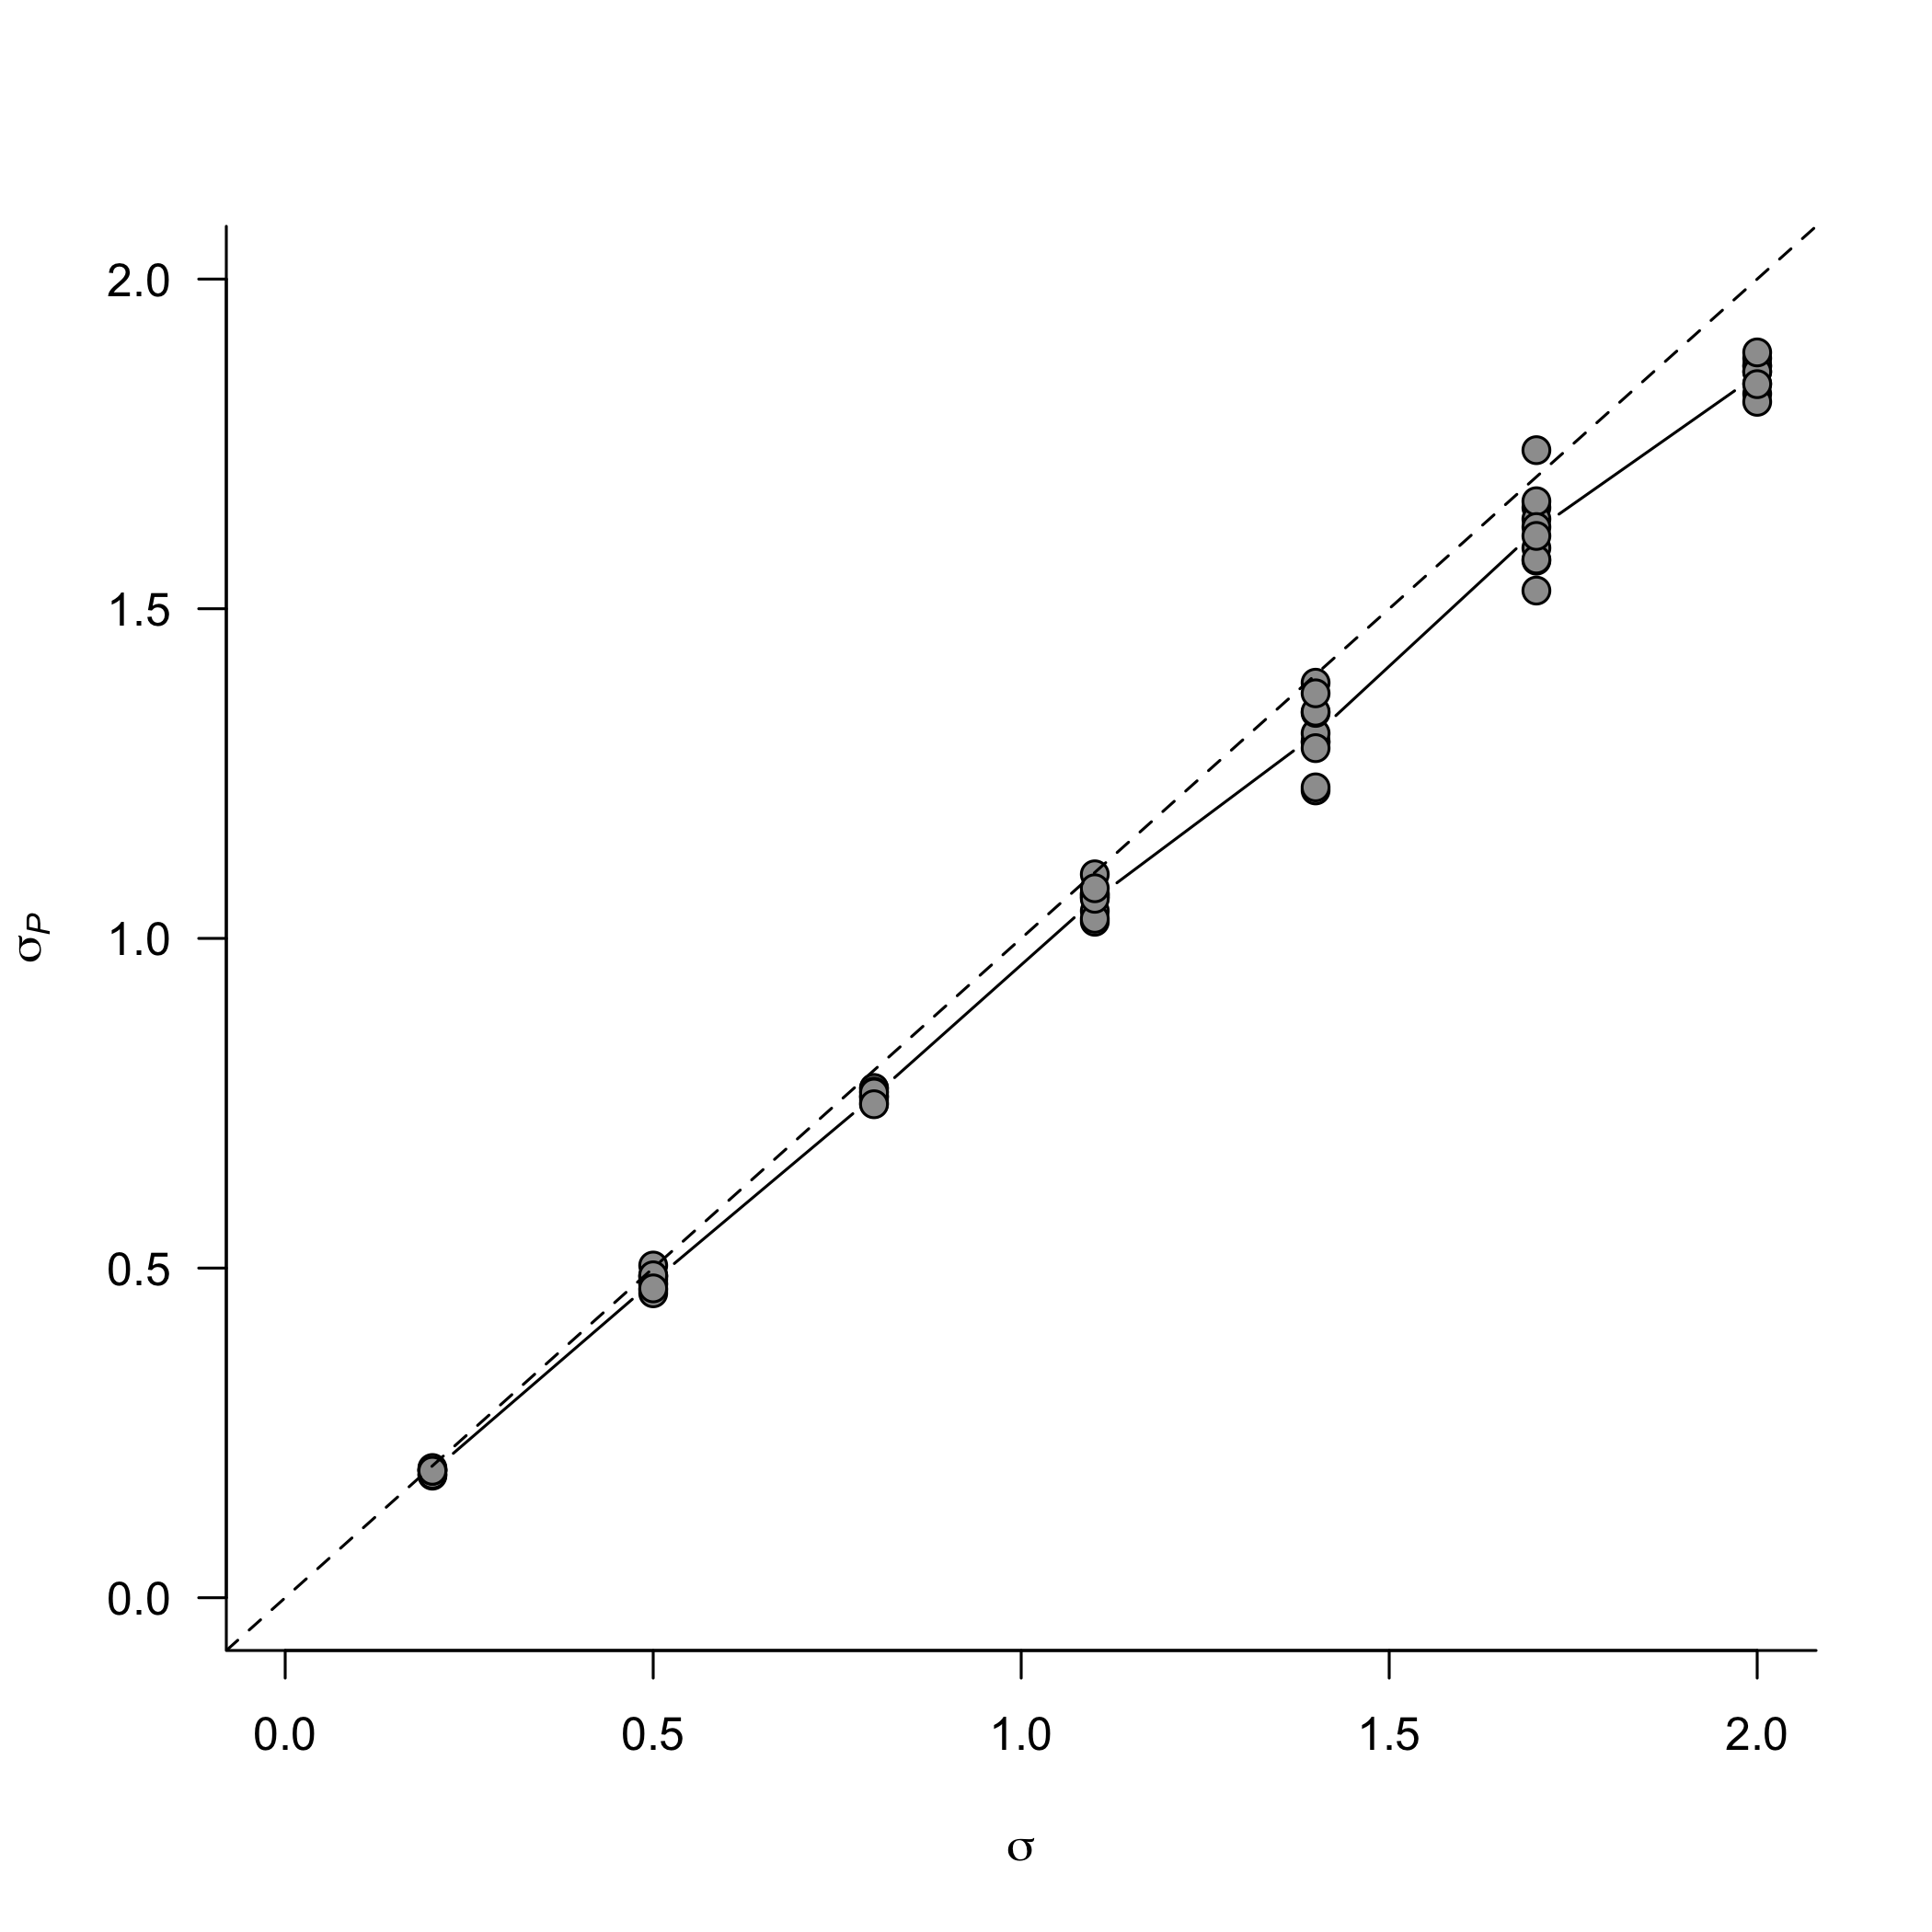
\includegraphics[width=\textwidth]{gauss-kernel-rate-estimates}
\caption{Migration rate estimates for a Gaussian dispersal kernel. Each point
represents a single simulation generated under Gaussian dispersal with effective
migration rate given on the x-axis and a parsimonious genome-wide estimate of that
rate on the y-axis. The inset line shows a 1:1 relationship.
}
\label{fig:gauss-kernel-rate-estimates}
\end{figure}

\begin{figure}[h]
\centering
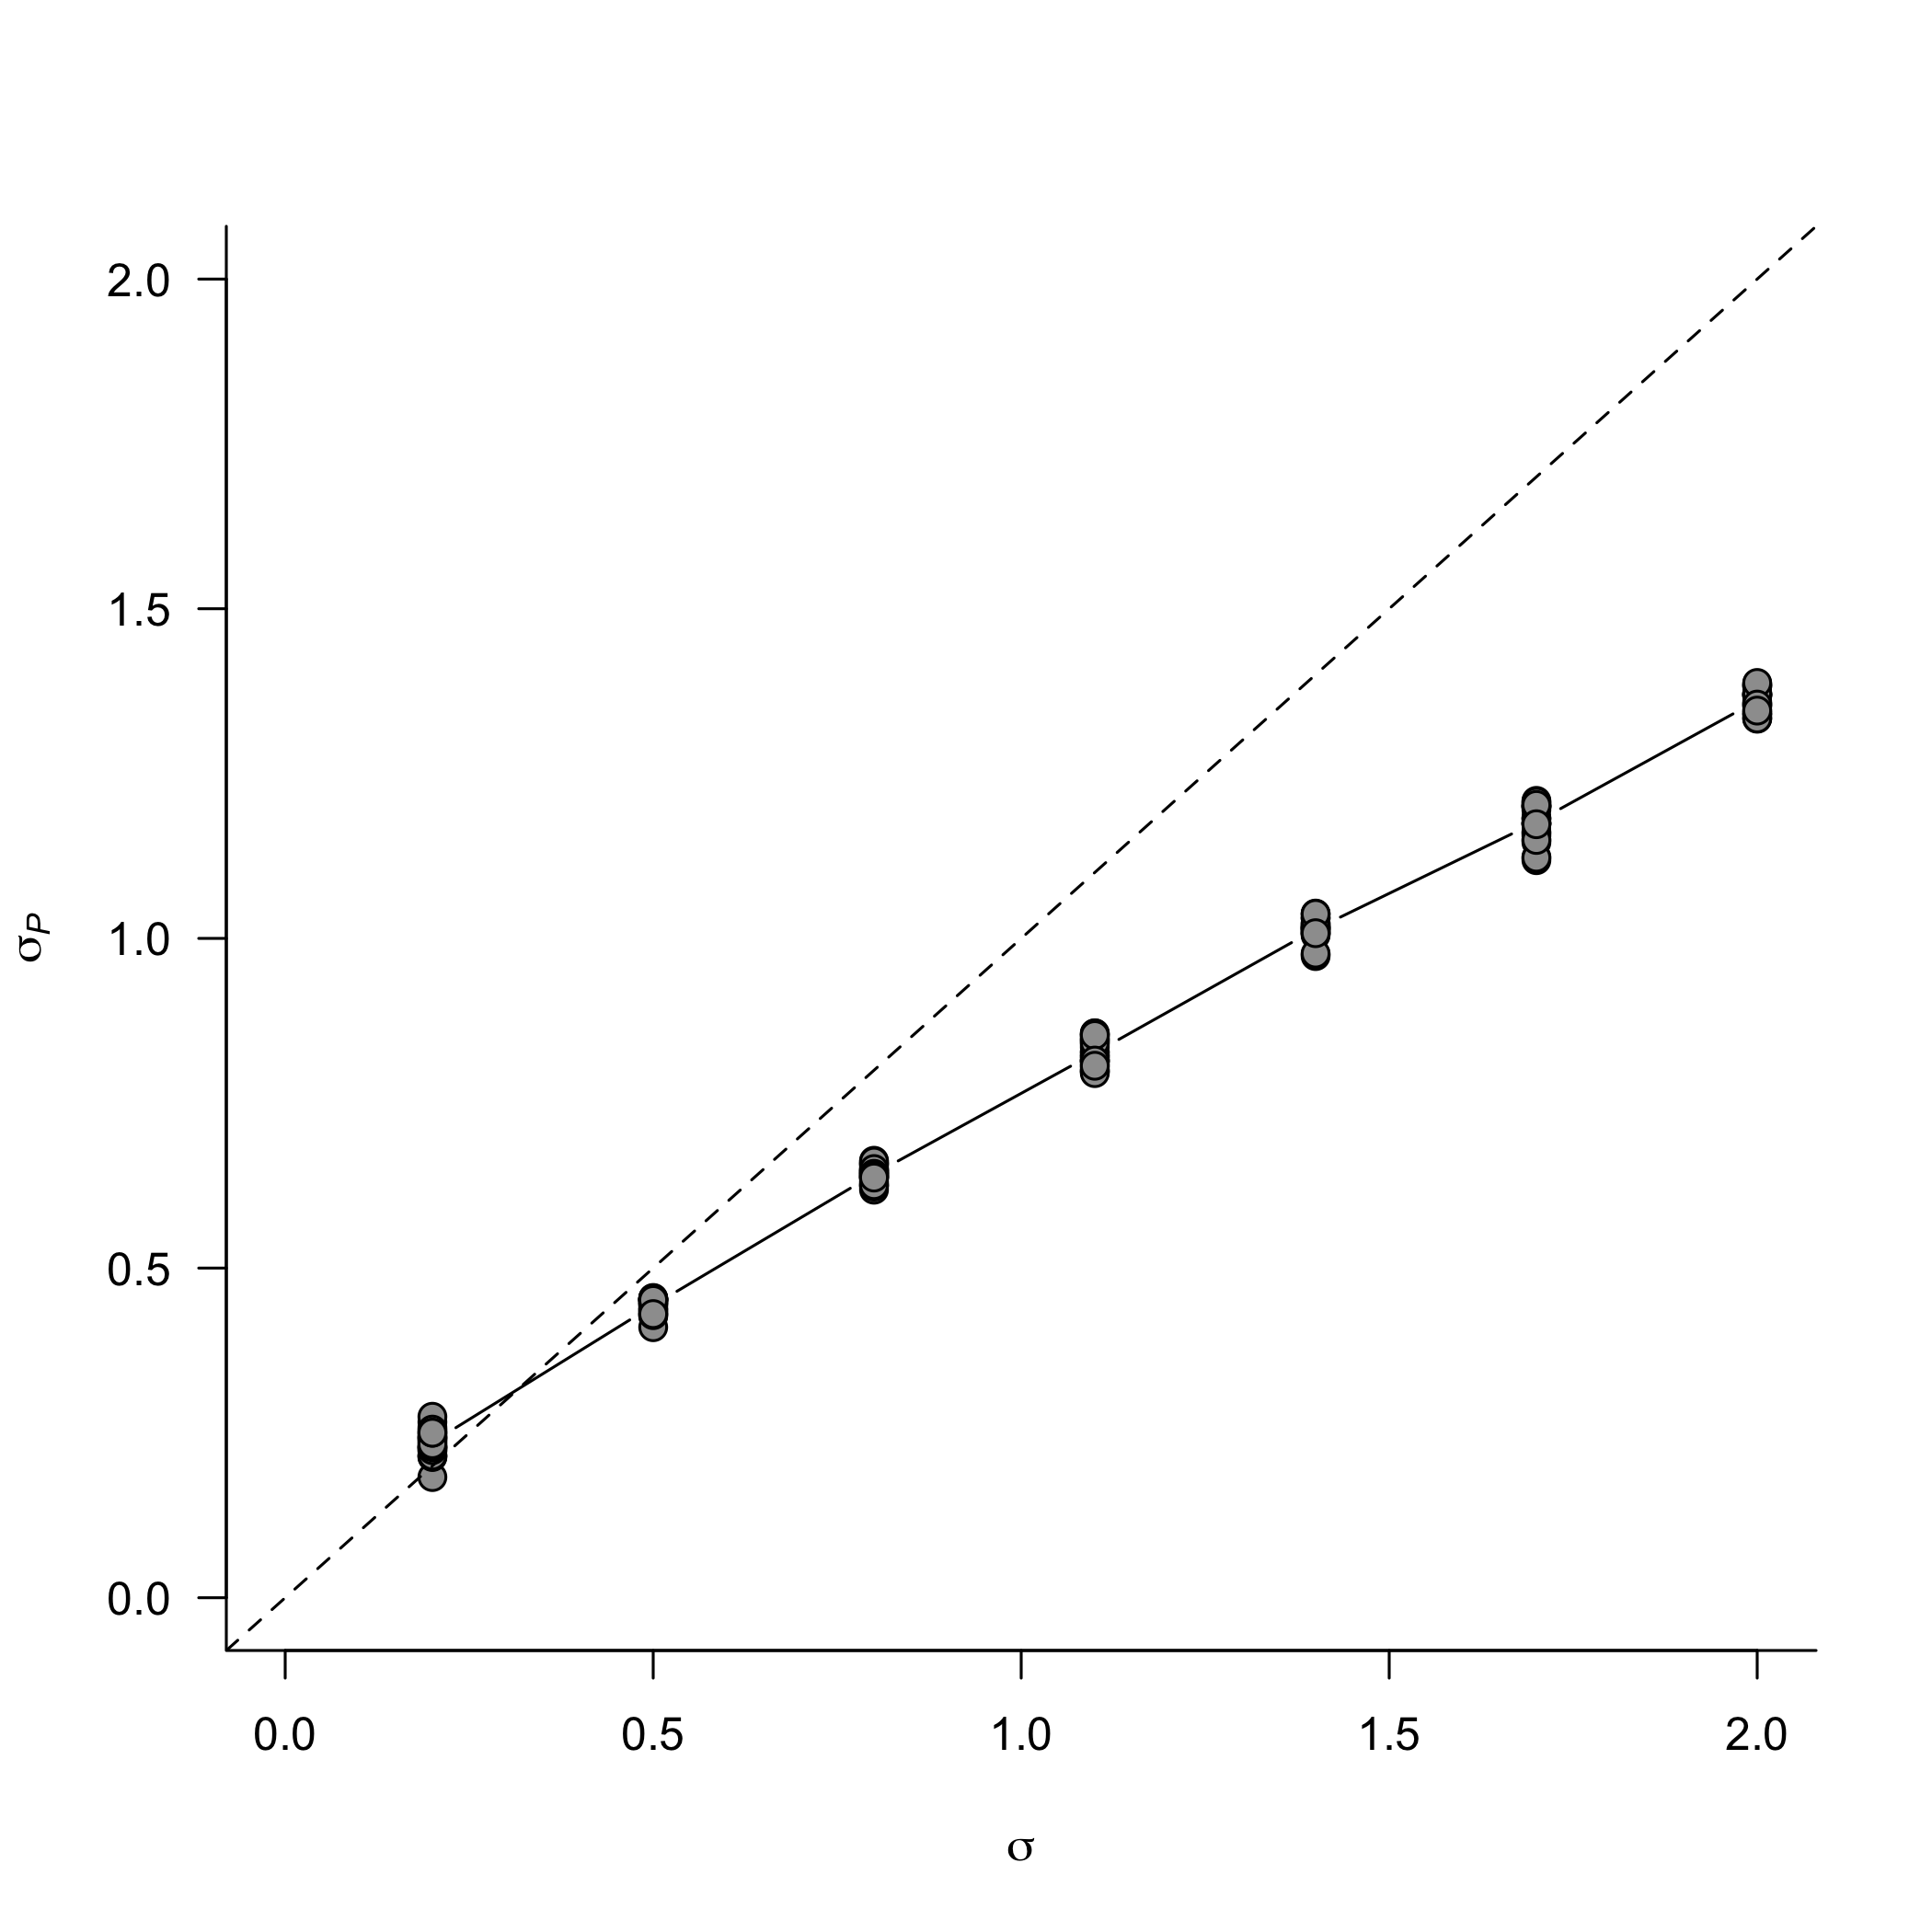
\includegraphics[width=\textwidth]{laplace-kernel-rate-estimates}
\caption{Migration rate estimates for a Laplace dispersal kernel. Each point
represents a single simulation generated under Laplace dispersal with effective
migration rate given on the x-axis and a parsimonious genome-wide estimate of
that rate on the y-axis. Estimates were conducted under three levels of 
discretization indicated by the color of the point (see main text).
The inset line shows a 1:1 relationship.
}
\label{fig:lapl-kernel-rate-estimates}
\end{figure}

\begin{figure}[h]
\centering
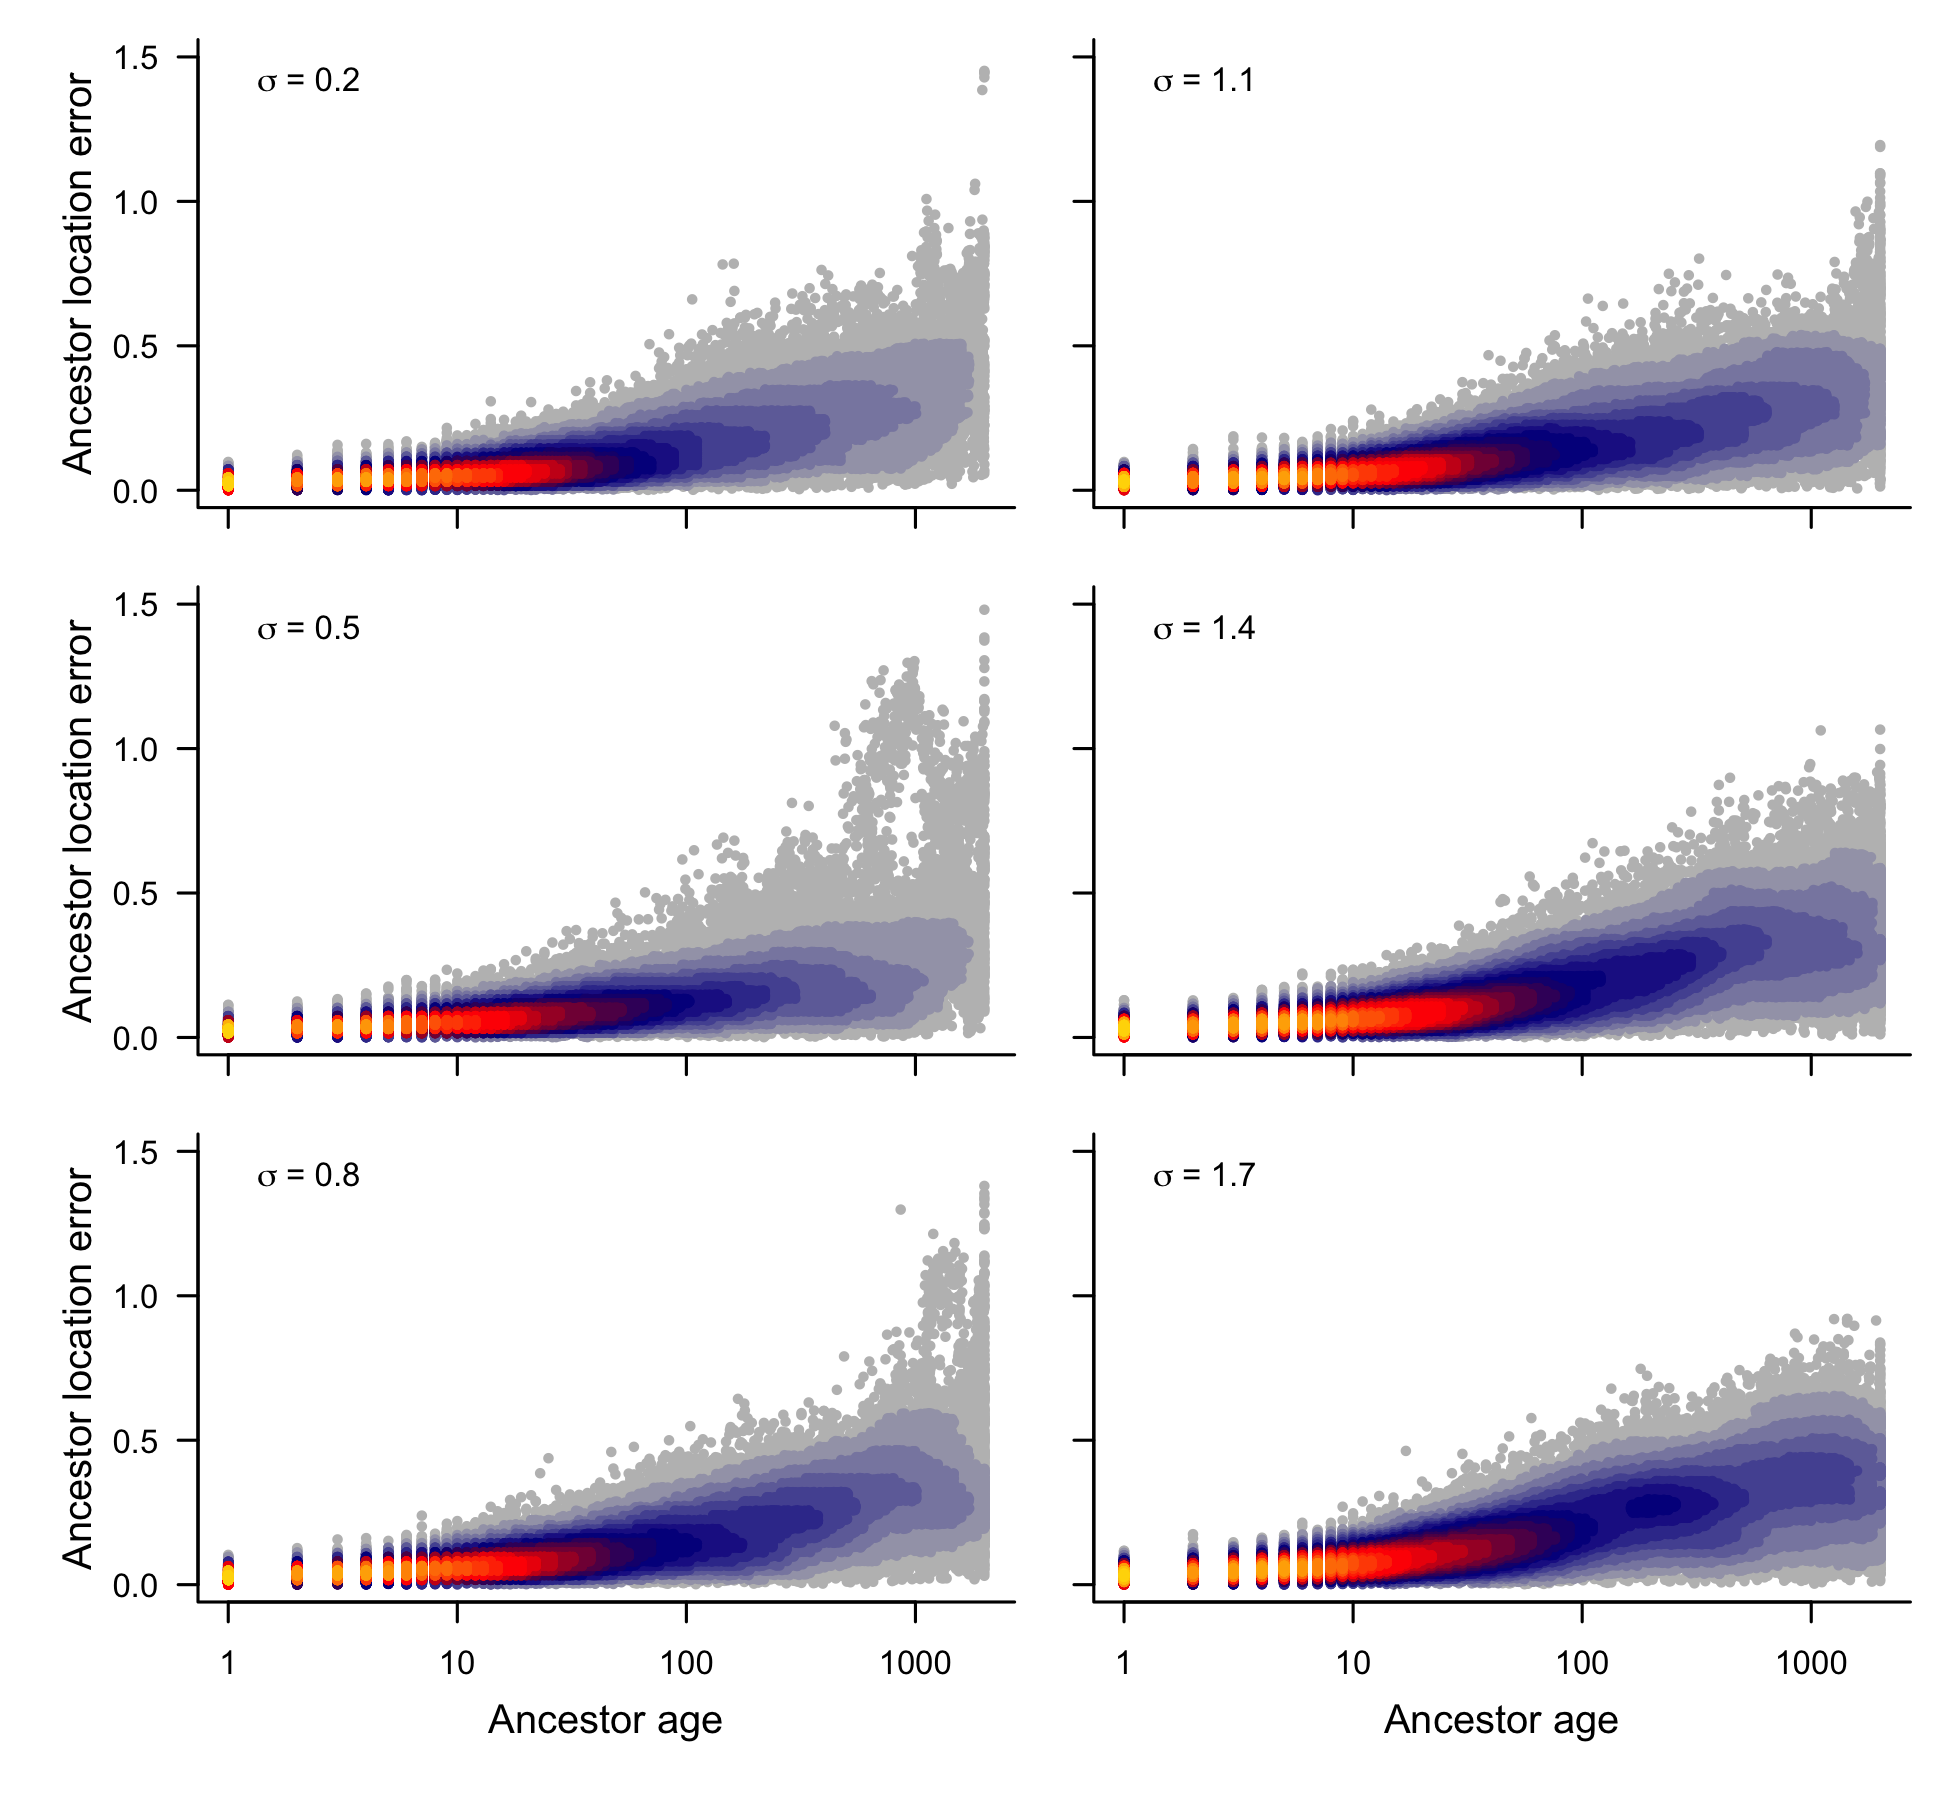
\includegraphics[width=\textwidth]{gauss-kernel-ancestor-estimates}
\caption{Ancestor location error for a Gaussian dispersal kernel. Each point
represents a single genetic ancestor. Ancestor location error is measured as
the distance between the estimated and the true location divided by the greatest
distance separating any pair of samples. Warm colors signify a greater density
of points.
}
\label{fig:gauss-kernel-ancestor-estimates}
\end{figure}

\begin{figure}[h]
\centering
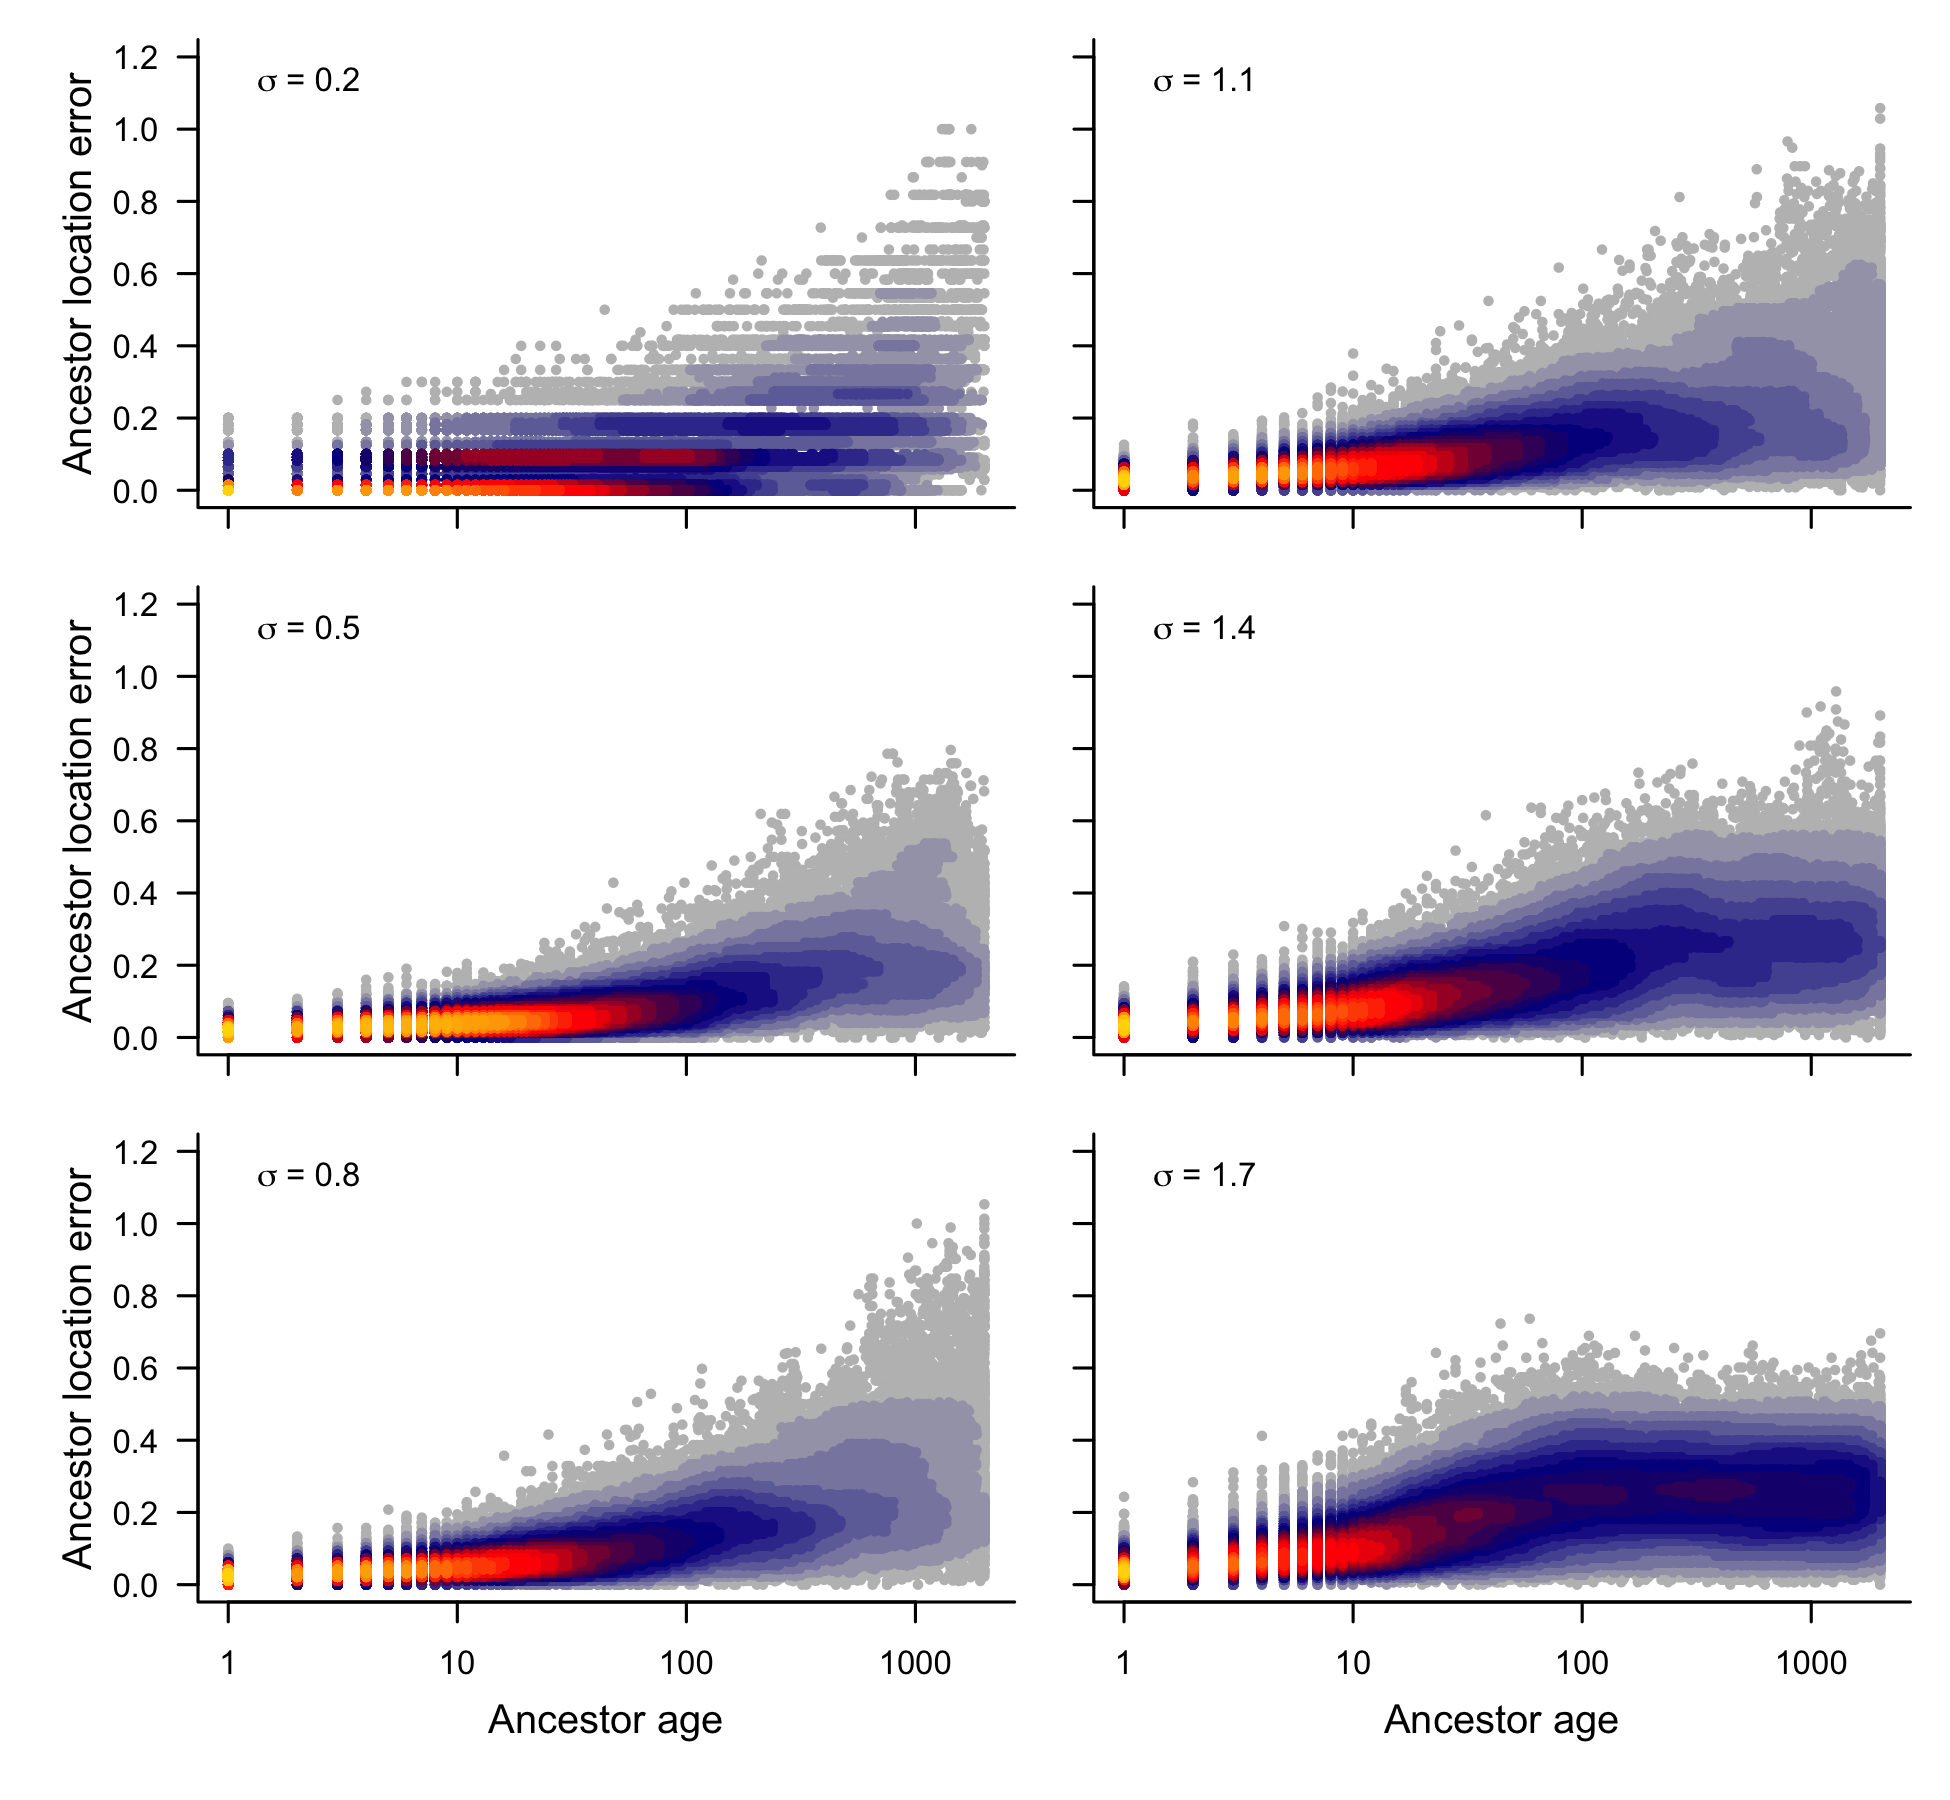
\includegraphics[width=\textwidth]{laplace-kernel-ancestor-estimates}
\caption{Ancestor location error for a Laplace dispersal kernel. Each point
represents a single genetic ancestor. Ancestor location error is measured as
the distance between the estimated and the true location divided by the greatest
distance separating any pair of samples. Warm colors signify a greater density
of points.
}
\label{fig:lapl-kernel-ancestor-estimates}
\end{figure}

\begin{figure}[h]
\centering
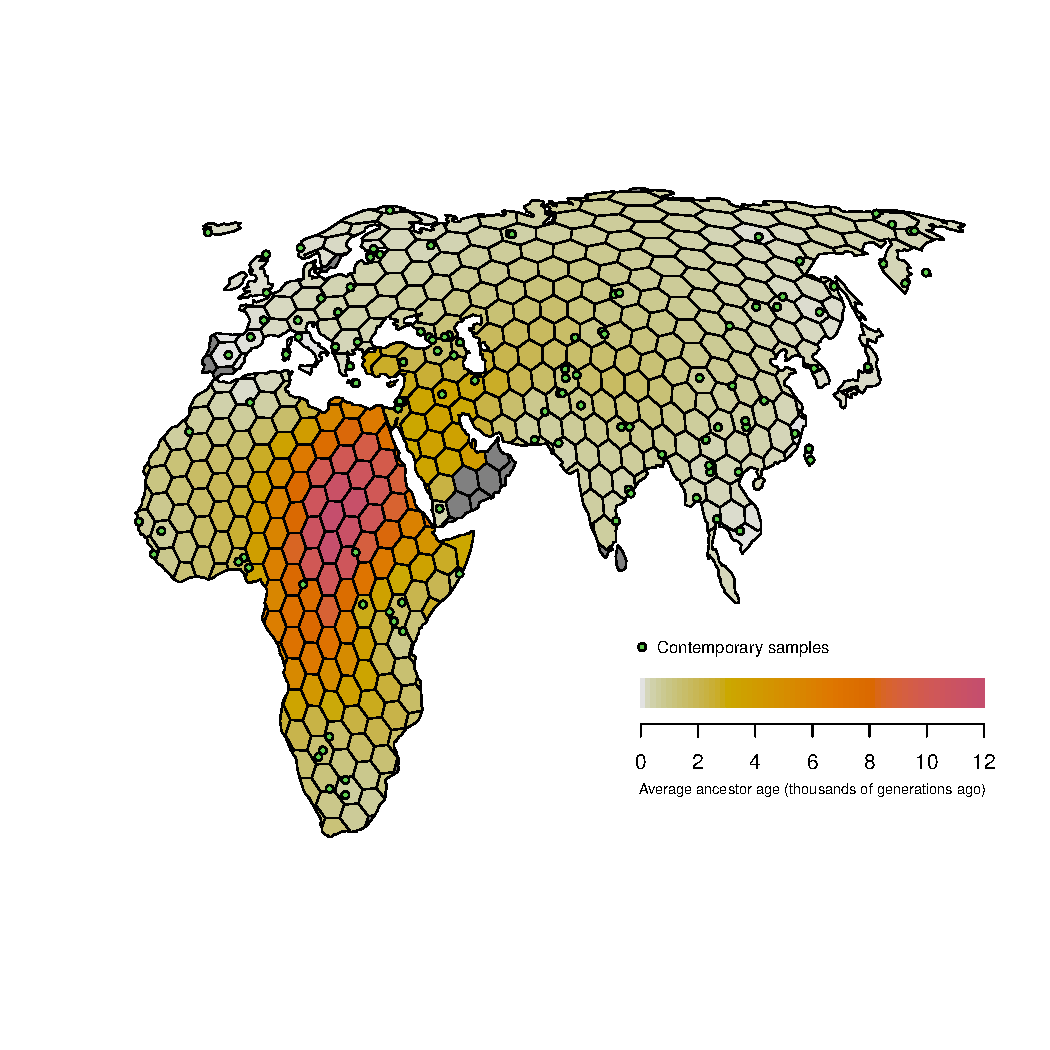
\includegraphics[width=\textwidth]{avg-ancestor-age}
\caption{Age distribution of genetic ancestors of contemporary human genome
samples. Every ancestor in the tree sequence is assigned a probability distribution 
over the set of grid cells reflecting its likely location. Each grid cell is 
colored by the weighted average of the ages of all genetic ancestors. Dark grey 
cells are omitted from the age distribution because the total weight of ancestors 
assigned to those cells is less than 1.}
\label{fig:avg-ancestor-age}
\end{figure}